\linespread{1.3}
\newgeometry{right=25mm,left=25mm,top=0mm,bottom=25mm}
\chapter{ INTRODUCTION}
\vspace{0.5cm}
In today’s world, cardiovascular diseases (CVDs) are one of the leading causes of mortality, claiming millions of lives every year. Early detection and timely monitoring of heart health are crucial for managing these conditions effectively. However, in many rural and remote areas, access to advanced healthcare facilities is limited, leaving a significant portion of the population at risk of undiagnosed heart conditions. Traditional multi-lead ECG machines, while effective, are expensive, bulky, and require trained professionals to operate\cite{Arias2016}. These challenges create a pressing need for an affordable, portable, and easy-to-use solution that can bring basic cardiac monitoring to the doorstep of every individual.

Imagine a scenario: A middle-aged farmer working in a rural area experiences occasional chest discomfort but dismisses it due to lack of access to medical facilities. One day, he suffers a major heart event because his condition went undetected for years. This is not just an isolated case but a recurring reality in underserved regions. What if there was a device that could have detected his heart condition earlier, allowing timely intervention?  

This project aims to address this critical gap by developing a single-lead, portable ECG machine. Our solution is compact, cost-effective, and user-friendly, making it ideal for rural and low-resource settings. The device is built using innovative DIY techniques, such as custom spiral copper wire electrodes, and powered by the AD8232 bioinstrumentation amplifier for reliable signal processing\cite{Parker2019}. The ESP8266 module enables wireless data transmission to any Wi-Fi-enabled device, offering a seamless user experience.  

Unlike traditional ECG systems, this project focuses on simplicity without compromising on diagnostic capabilities. The captured ECG data is displayed on a web interface in real-time, making it accessible to both healthcare professionals and individuals for personal monitoring. With its focus on affordability, mobility, and functionality, this device has the potential to revolutionize cardiac care in rural areas, promoting better health outcomes.  

\newgeometry{right=25mm,left=25mm,top=20mm,bottom=25mm}


\chapter{BACKGROUND}
The heart is mainly a muscle that requires a stimulus in order to beat and pump blood into the body. This stimulus comes in the form of electric pulses emitted by the sinoatrialnode, a grouping of specialised cells located in the top right hand corner of the heart. Pulses are produced periodically thus maintaining the beating of the heart. They can, - as it will be explained later in the report - if captured and plotted,help physicians diagnose the heart they originated from. The Electrocardiogram fulfils this purpose and has been used to do so for more than a century. 
\begin{figure}[H]
    \centering
    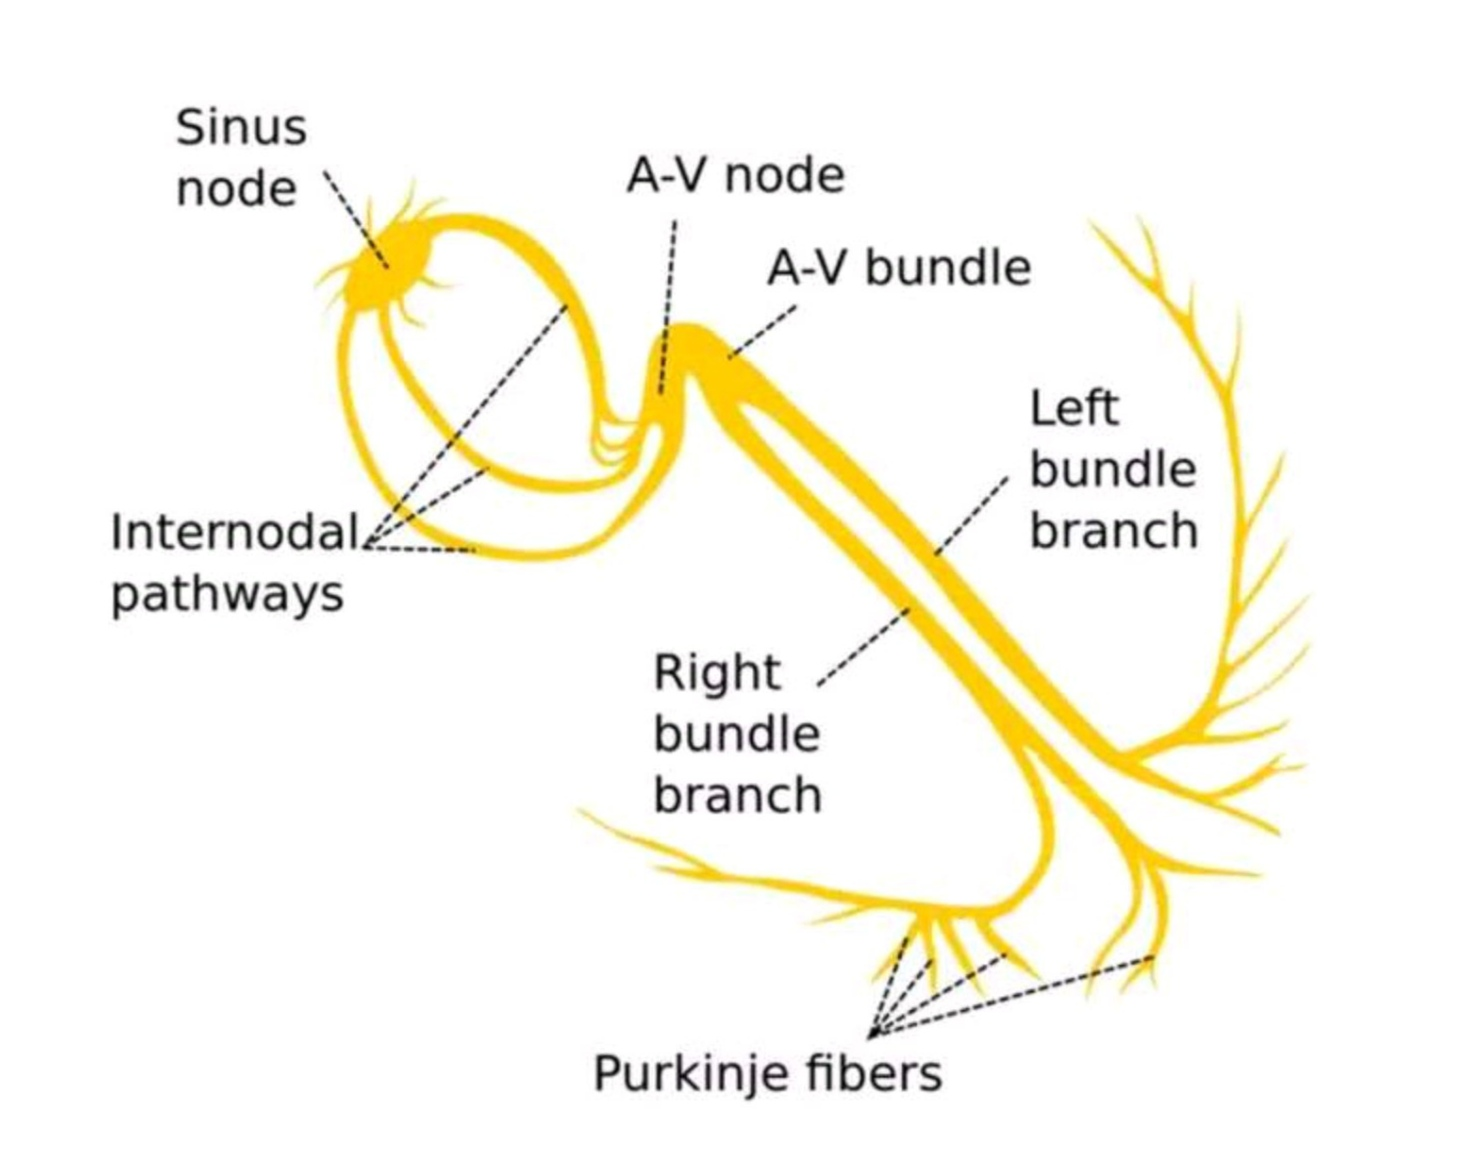
\includegraphics[scale=0.1]{images/electrical_heart.jpg}
    \caption{The electrical conduction system of the heart}
    \label{fig:electrical_heart}
\end{figure}
The electrical pulse generated has a unique pattern (seen in \autoref{fig:pqrst}), it includes many significant waves that concern different parts of the heart\cite{Kiani2018}.
\begin{figure}[H]
    \centering
    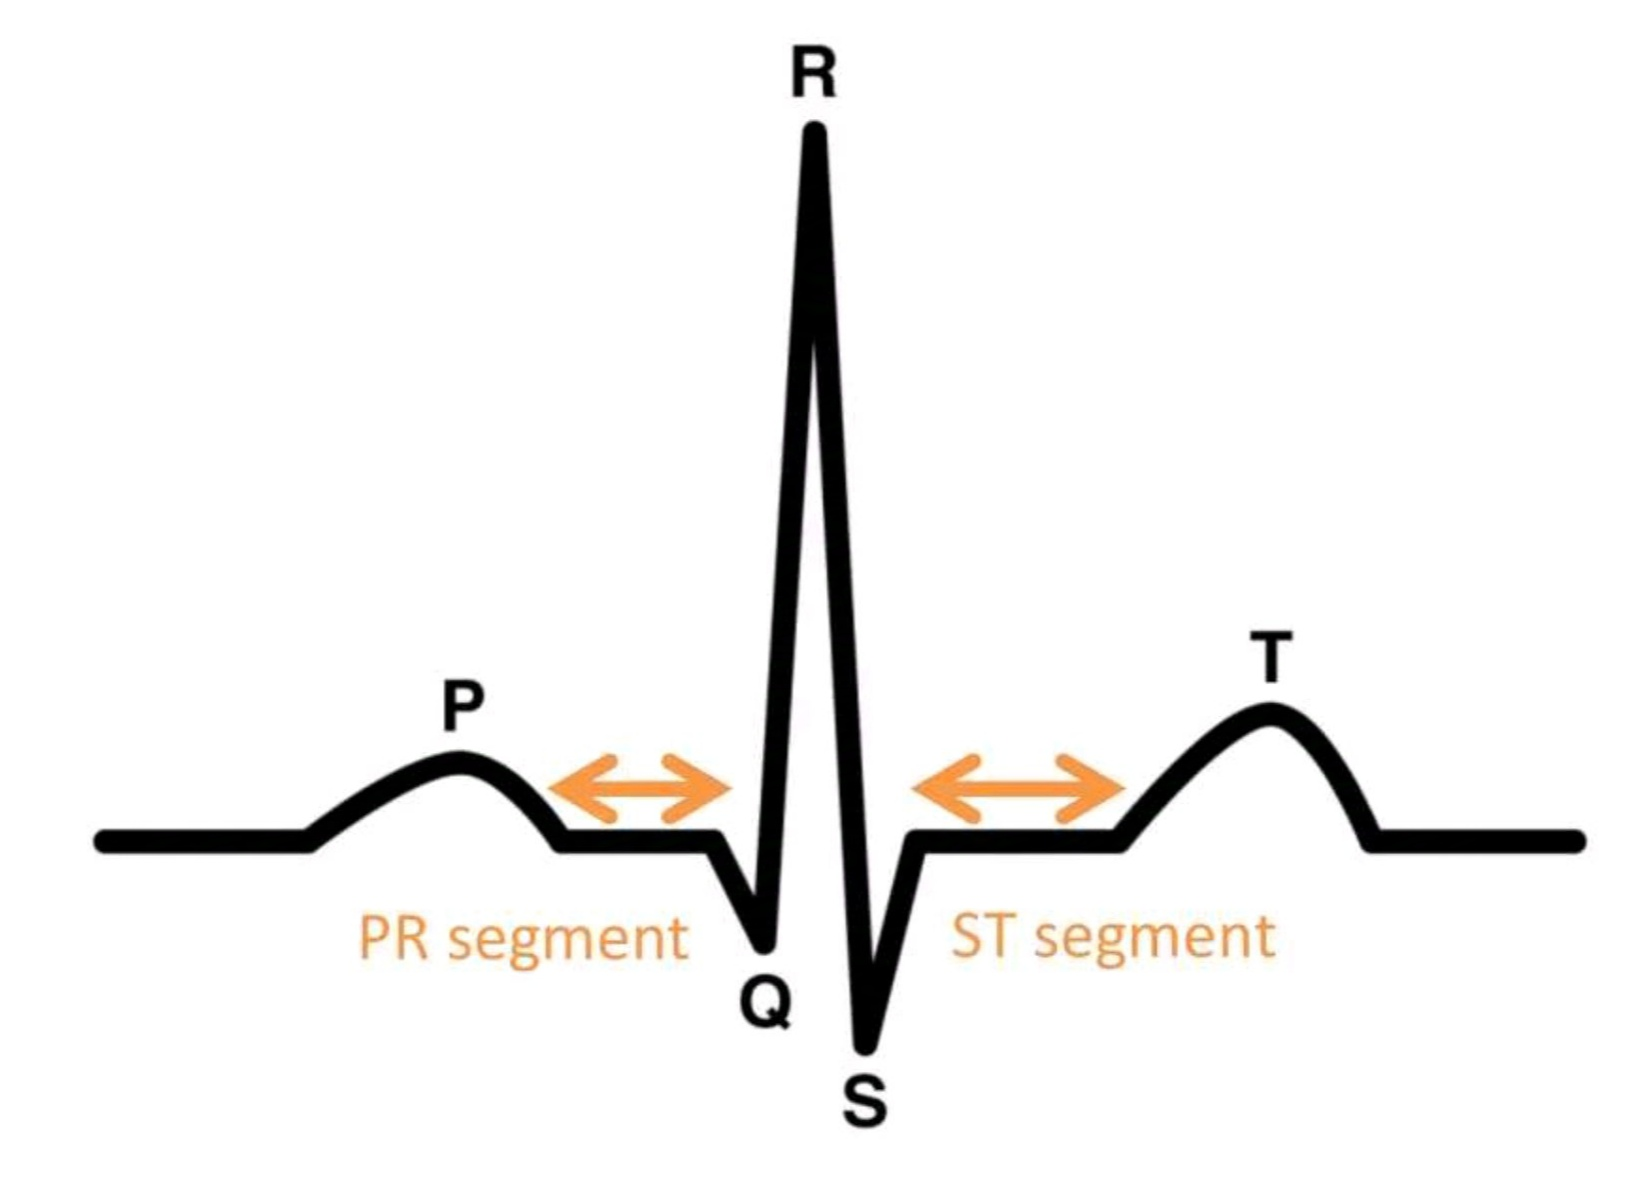
\includegraphics[scale=0.1]{images/pqrst.jpg}
    \caption{Normal ECG signal pattern}
    \label{fig:pqrst}
\end{figure}
Multi-lead ECG machines are commonly used in medical settings but have notable limitations for rural healthcare. They are not only costly but also complex to operate, maintain, and interpret. This complexity, combined with high expenses, restricts accessibility in rural or remote areas where resources and trained personnel are scarce. Recognizing these barriers, our project focuses on creating a simplified, single-lead ECG device that can make essential cardiac monitoring accessible to everyone.
\begin{figure}[H]
    \centering
    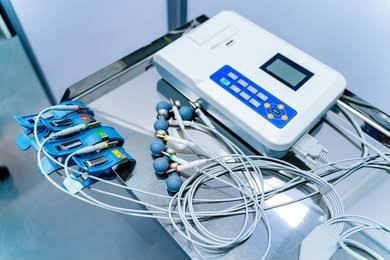
\includegraphics[scale=1]{images/hospital_ecg.jpg}
    \caption{Traditional Hospital ECG Machine}
    \label{fig:hospital_ecg}
\end{figure}



\chapter{PROPOSED DESIGN}
After having completed the background research on the type of signal that will have to be picked up by the ECG monitor to be built, it was decided that the project's ECG monitor would be a two or three electrode ECG powered by one 3.7 V battery. A few design specifications were set in order to ensure proper ECG signal sampling.

\begin{figure}[H]
    \centering
    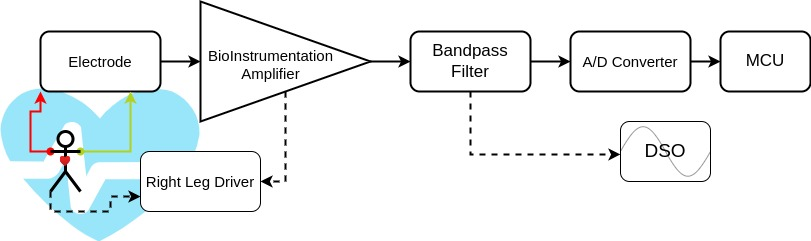
\includegraphics[scale=0.5]{images/ecg_block_diagram.jpg}
    \caption{ECG block diagram}
    \label{fig:ecg_block_diagram}
\end{figure}

\section{ELECTRODES}
To reduce costs and improve accessibility, we designed custom electrodes using copper wires bent into a spiral shape (see in \autoref{fig:electrodes})\, approximately the size of a finger. This spiral structure ensures adequate skin contact, allowing for stable electrical signal acquisition. These DIY electrodes are reusable, simple to construct, and effective for single-lead ECG applications.
\begin{figure}[H]
    \centering
    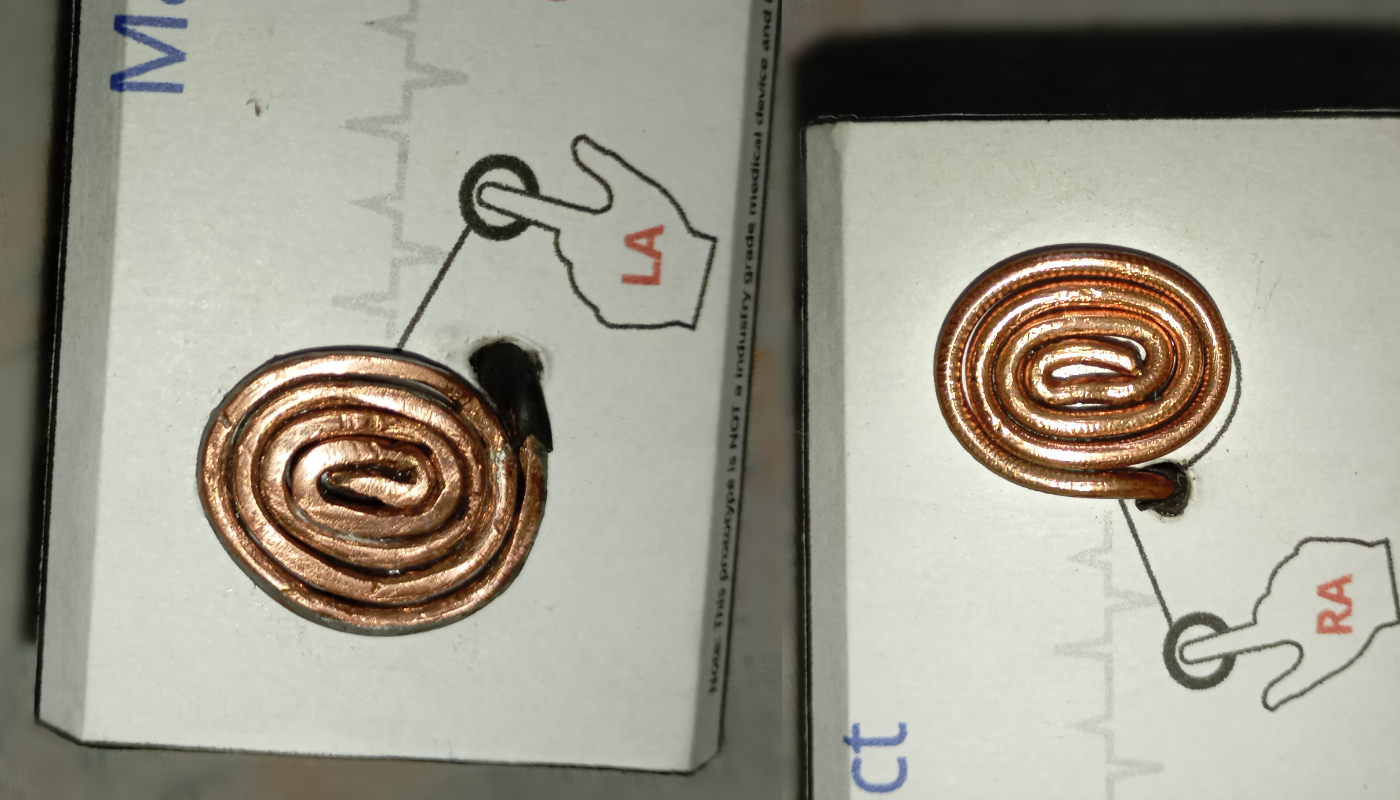
\includegraphics[scale=3]{images/electrode.jpg}
    \caption{DIY reusable electrodes}
    \label{fig:electrodes}
\end{figure}


\section{AMPLIFIER}
We use the AD8232\cite{AD8232} bioinstrumentation amplifier, a reliable choice for portable ECG devices. This amplifier is designed to capture the heart’s weak electrical signals and amplify them for accurate processing. It offers high precision, low power consumption, and effective signal enhancement, making it suitable for mobile applications where battery efficiency and signal clarity are crucial.
\begin{figure}[H]
    \centering
    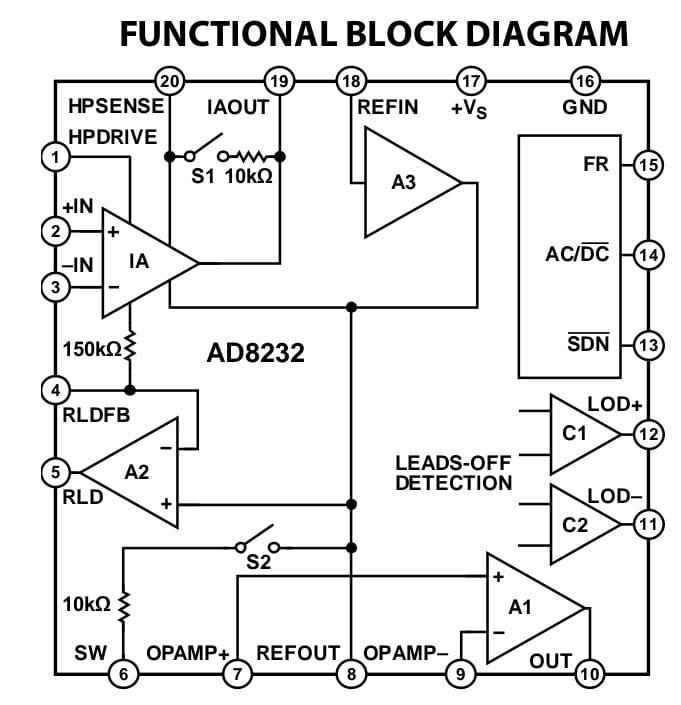
\includegraphics[scale=0.3]{images/ad8232_block.jpg}
    \caption{AD8232 block diagram\cite{AD8232}}
    \label{fig:AD8232_block}
\end{figure}

\section{NOISE \& FILTER}
Noise in the ECG system can originate from multiple sources, such as electromagnetic interference from power lines, motion artifacts due to user movement, and baseline wander caused by respiration. The AD8232 module integrates built-in filters to address high-pass and low-pass noise, reducing complexity. For additional filtering, an RC filter can be added at critical stages to further attenuate power line noise or other interference\cite{Tayal2018}.


\section{DSO}
We have implemented a DIY Digital Storage Oscilloscope using the ESP8266\cite{Espressif2015} microcontroller with WiFi capabilities. This module captures the processed ECG signal and allows for real-time visualization in any of your wifi enabled device. Unlike traditional DSOs, this DIY approach is cost-effective, compact, and customizable. The ESP8266’s WiFi functionality also supports remote monitoring, enabling healthcare providers to view ECG data without physical contact—a significant advantage for rural and telemedicine applications.

\begin{figure}[H]
    \centering
    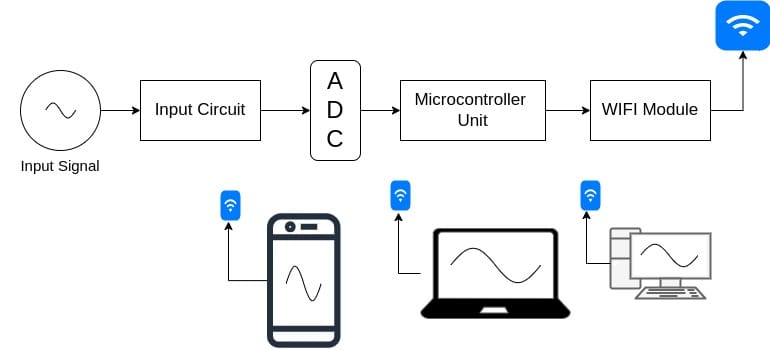
\includegraphics[scale=0.5]{images/dso_block_diagram.jpg}
    \caption{DSO block diagram}
    \label{fig:dso_block_diagram}
\end{figure}

\section{WIFI}
The ESP8266\cite{Espressif2015} MCU provides built-in Wi-Fi connectivity for transmitting ECG data to nearby devices. The system take advantage of HTTP or WebSocket protocols for efficient real-time data streaming. This ensures users can view ECG signals wirelessly on a smartphone, PC or any other wifi enabled device with working browser, enabling mobile diagnostics.




\chapter{Software Development}

Capture analog ECG signals in MCU, process them, and transmit data wirelessly to a user interface maybe a webpage for real-time visualization\cite{Wang2017}.
\begin{algorithm}
\addcontentsline{toc}{section}{Microcontroller programming Algorithm}
\caption{Microcontroller programming Algorithm}
\begin{algorithmic}[1]
\STATE \textbf{Initialize:}
\STATE Initialize Serial Communication for debugging
\STATE Initialize Wi-Fi as Access Point
\STATE Configure DNS Server
\STATE Configure WebSocket Server
\STATE Configure Web Server Routes

\WHILE{True}
    \STATE \textbf{Handle WebSocket Events:}
    \IF{Message Type = \texttt{WStype\_TEXT}}
        \STATE Extract message data
        \STATE Parse the message
        \STATE Collect sensor readings
        \STATE Prepare and send response to client
    \ENDIF
    \IF{Message Type = \texttt{WStype\_CONNECTED}}
        \STATE Log connection details
    \ENDIF
    \IF{Message Type = \texttt{WStype\_DISCONNECTED}}
        \STATE Log disconnection details
    \ENDIF
\ENDWHILE
\end{algorithmic}
\end{algorithm}

\begin{algorithm}
\addcontentsline{toc}{section}{Web Development Algorithm}
\caption{Web Development Algorithm (User Interface)}
\begin{algorithmic}[1]
\STATE \textbf{Initialize:}
\STATE \quad Initialize an empty buffer \texttt{data\_buffer} with a predefined size (e.g., 2000)
\STATE \quad Set up WebSocket connection to receive incoming data from the MCU\cite{WebSocketAPI2024}

\STATE \textbf{On WebSocket Connection Open:}
\STATE \quad Display success notification "Connection established!"
\STATE \quad Send a signal (1) to the WebSocket server to request data

\STATE \textbf{On Receiving Data:}
\STATE \quad Parse the incoming data
\STATE \quad Append the received data to \texttt{data\_buffer}
\STATE \quad Trim the \texttt{data\_buffer} to maintain a fixed length (e.g., the number of elements corresponding to the canvas width)
\STATE \quad Send a signal (200) to the server indicating successful data reception

\STATE \textbf{Auto Scale Function:}
\STATE \quad Calculate the scale factor for voltage (\texttt{volt\_per\_div}) using the difference between the maximum and minimum values in \texttt{data\_buffer}
\STATE \quad Adjust the vertical position (\texttt{positionY}) to center the data values in the middle of the canvas
\STATE \quad Update the UI with the new scale factor and position values

\STATE \textbf{Graph Drawing Loop:}
\STATE \quad Clear the canvas area to prepare for a new drawing
\STATE \quad Call the function to draw graph axes
\STATE \quad Begin plotting the graph:
\STATE \quad \quad For each point in \texttt{data\_buffer}:
\STATE \quad \quad \quad Calculate the corresponding x and y coordinates on the canvas based on the time per division (\texttt{time\_per\_div}) and voltage per division (\texttt{volt\_per\_div})
\STATE \quad \quad \quad Plot the calculated point on the canvas
\STATE \quad \quad End the line when the graph reaches the end of the canvas

\STATE \textbf{Draw Graph Axes:}
\STATE \quad Draw horizontal and vertical grid lines based on the time and voltage divisions
\STATE \quad Label the axes with appropriate markers (e.g., time and voltage values)

\STATE \textbf{Resize Event Handling:}
\STATE \quad Adjust the canvas width and reset the data buffer size based on the screen width

\STATE \textbf{Touch Event Handling:}
\STATE \quad Track touch input on the canvas and update the pointer position based on user interaction (for example, tracking voltage or time)

\STATE \textbf{Notification System:}
\STATE \quad Display WebSocket status notifications (success, error, warning) with appropriate colors and auto-hide functionality

\end{algorithmic}
\end{algorithm}


\newgeometry{right=25mm,left=25mm,top=0mm,bottom=25mm}
\chapter{Implementation and Results}
\begin{figure}[H]
    \centering
    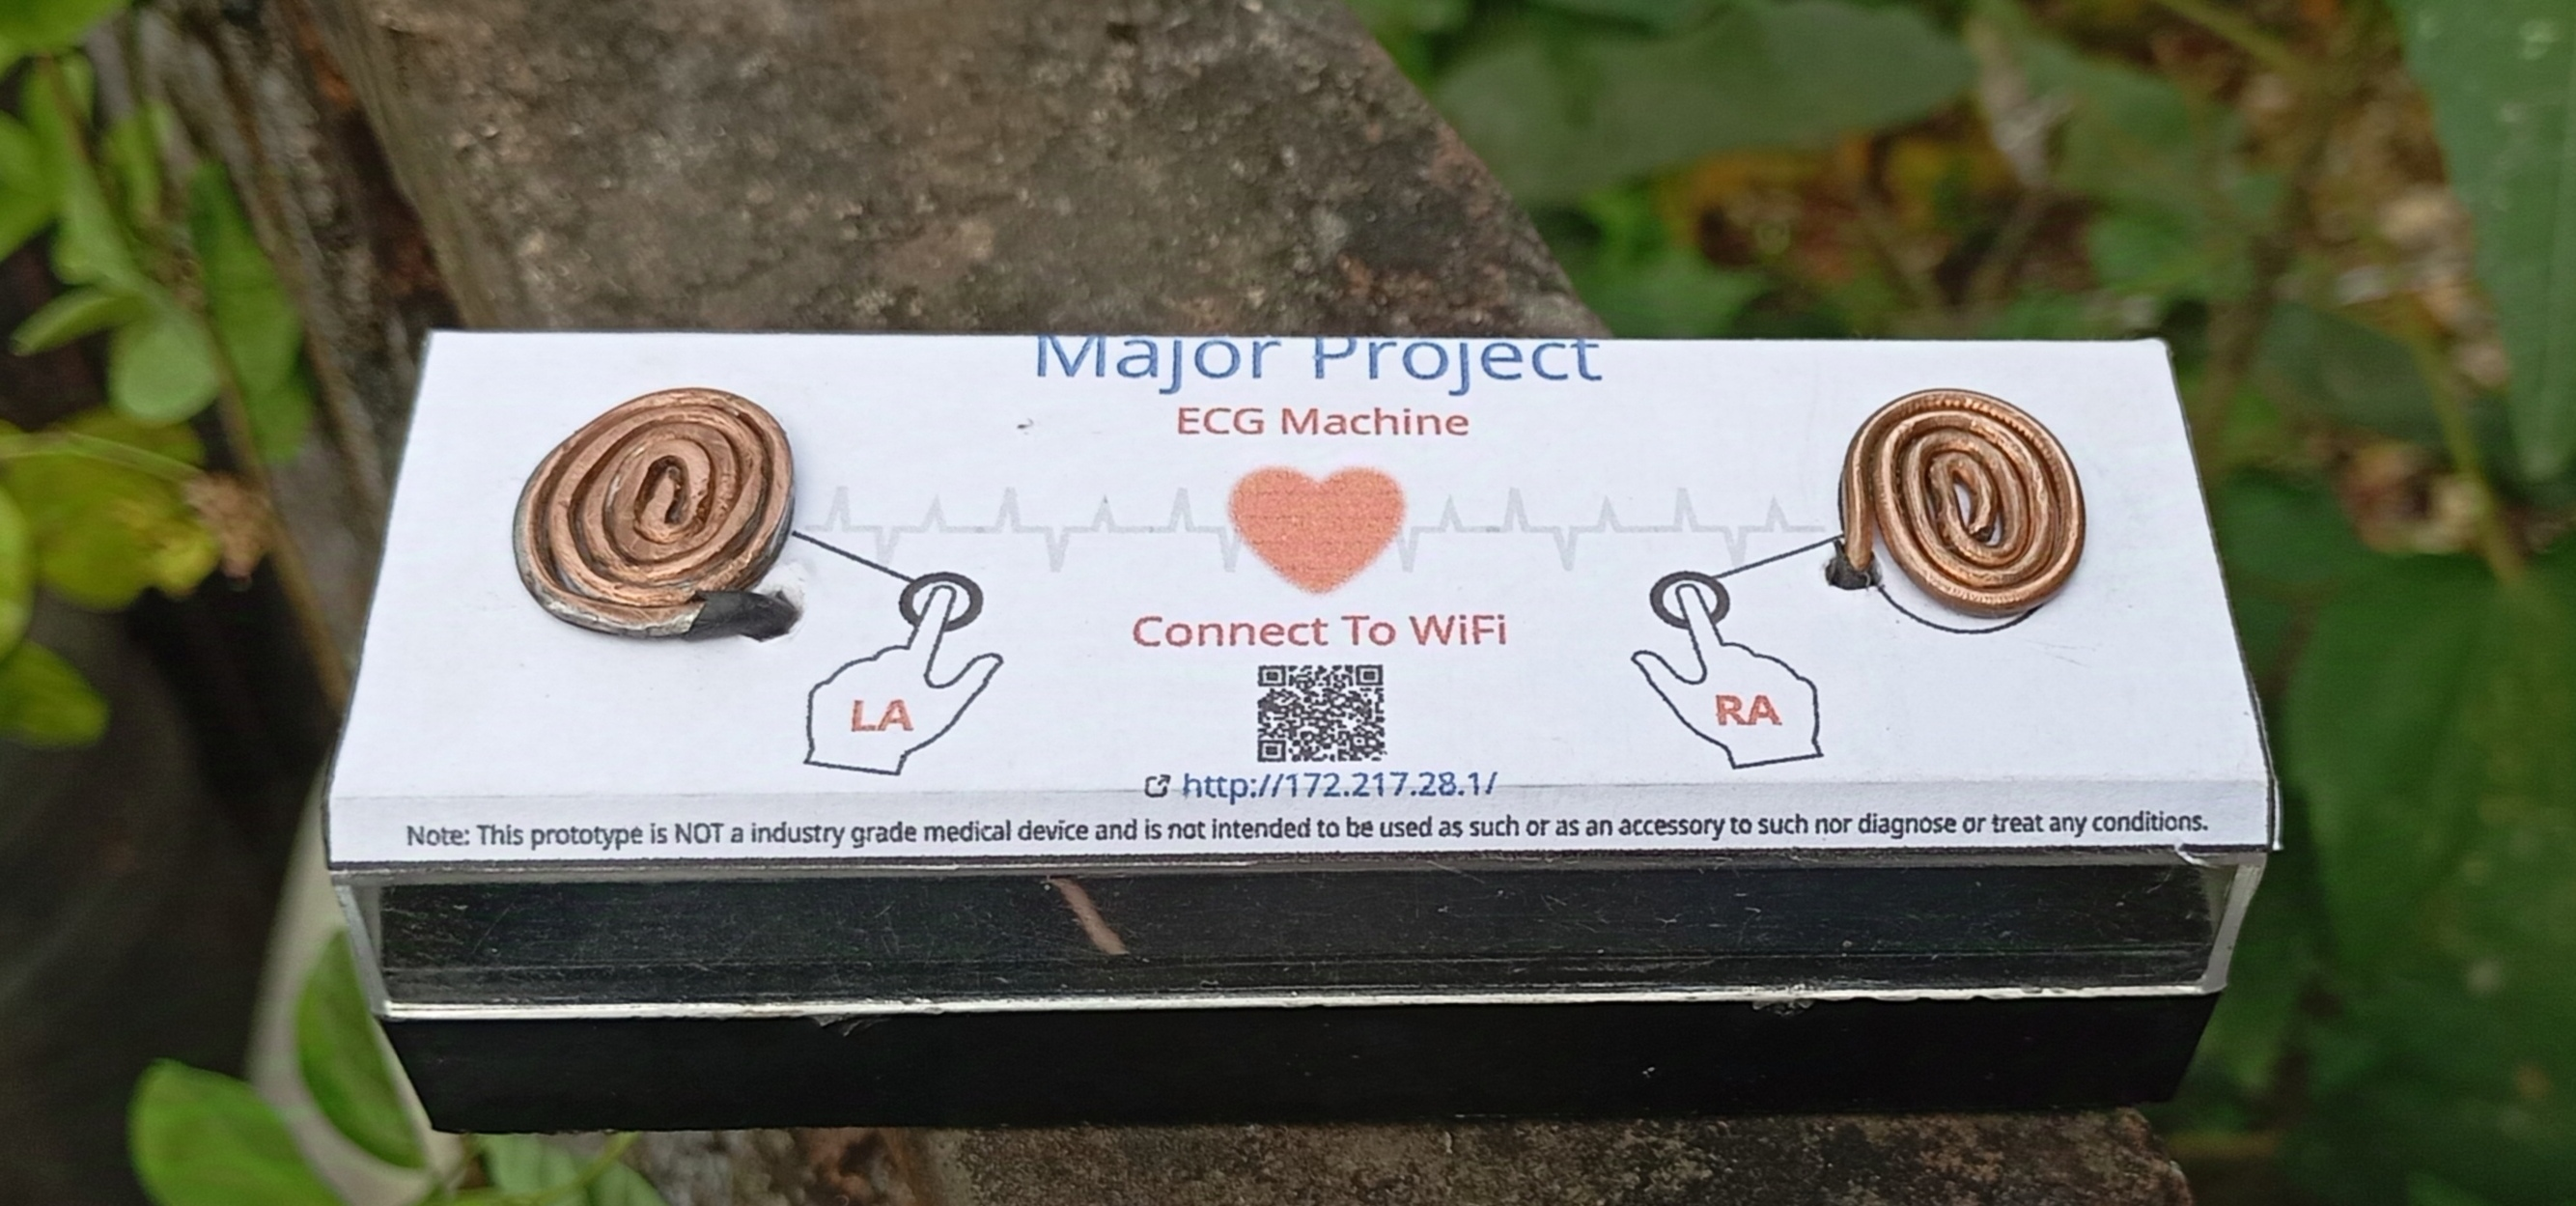
\includegraphics[scale=0.1]{images/proto.jpg}
    \caption{Project Prototype, implemented the entire circuit inside the box}
    \label{fig:proj_proto}
\end{figure}
\begin{figure}[H]
    \centering
    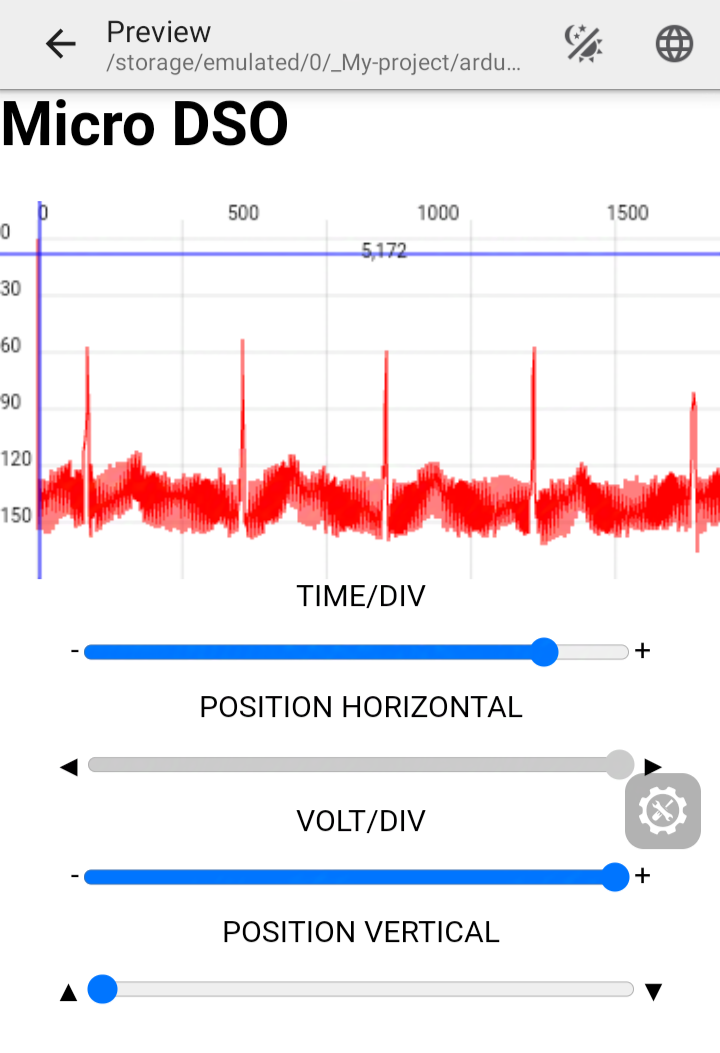
\includegraphics[scale=0.3]{images/result.png}
    \caption{User interface with Project result or output}
    \label{fig:proj_result}
\end{figure}
\newgeometry{right=25mm,left=25mm,top=20mm,bottom=25mm}


\chapter{Future Scope}

The portable single-lead ECG machine is a big step toward making heart health check-ups available to everyone, especially in areas where healthcare is hard to access. While the current design works well for basic monitoring, there is a lot of room to improve and add new features in the future. Below are some ideas for what could be done next:

\section{Artificial Intelligence (AI) Features}
Adding AI to the device can help it automatically detect heart problems like irregular heartbeats. Using machine learning models as discussed in previous research \cite{Kiani2018}, this feature would make the device useful even for people who don’t have medical training.

\section{Multi-Lead ECG Option}
Right now, the machine uses a single lead, which works for basic monitoring. In the future, it can be upgraded to include more leads, which would make it better for detailed heart check-ups and more complex diagnoses \cite{Arias2016}.

% \section{Better Connectivity}
% Currently, the device uses Wi-Fi for sending data. Adding other options like Bluetooth or mobile data (4G/5G) can make it work in areas where Wi-Fi isn’t available. Similar approaches have been implemented in other wireless ECG systems \cite{Wang2017}.

\section{Improving Signal Quality}
The ECG machine can be improved by using advanced filtering techniques to reduce noise, such as motion artifacts or interference from other electrical devices. Techniques like precision filters and real-time noise reduction \cite{Tayal2018} would help provide clearer and more accurate heart signals for analysis.

\section{Data Logging}
Adding a data logging feature would allow users to save their ECG recordings for future reference. This could help doctors track a patient’s heart health over time and identify any long-term changes. Data storage capabilities using IoT modules like ESP8266 have been explored in similar devices \cite{Espressif2015}.

\section{Remote Monitoring}
This machine could be connected to telemedicine apps so doctors can monitor patients from far away in real time. This feature aligns with global trends in telemedicine \cite{Arias2016}, enabling quicker responses to emergencies and better care for rural populations.

\section{Customizable Features}
The device could include options for users to adjust the settings based on their needs, such as monitoring for children or older adults. A user-friendly interface, as implemented in this project, could be further refined to suit a wider range of users \cite{Mozilla2024}.

\section{Support for Rural Healthcare Programs}
Working with organizations and governments, this device could be made available to more people in remote areas. This would help ensure that everyone, no matter where they live, can check their heart health easily. Affordable healthcare technologies, like this ECG machine, have a proven impact on improving health equity \cite{Parker2019}.

These improvements would make the single-lead ECG machine even more useful and impactful, helping more people take care of their heart health in a simple and affordable way.



\chapter{CONCLUSION}
The development of a portable, single-lead ECG machine demonstrates the potential for affordable and accessible cardiac monitoring solutions, particularly for underserved rural and remote areas. By utilizing custom-built spiral copper electrodes, the AD8232 bioinstrumentation amplifier, and the ESP8266 Wi-Fi module, the project successfully achieves real-time ECG signal acquisition, processing, and wireless data transmission.

\vspace{0.8cm}
The integration of a user-friendly web interface for ECG visualization ensures that the system is practical and convenient for non-specialist users. Field testing has shown that the device performs reliably, with comparable accuracy to standard ECG machines, while significantly reducing costs. This prototype bridges a critical gap in rural healthcare by providing an essential diagnostic tool for early detection and management of cardiac conditions.

\vspace{0.8cm}
Future enhancements could include the incorporation of multi-lead functionality, AI-driven data analysis, and extended battery life. This project highlights the significant impact that low-cost healthcare technologies can have on improving global health equity.

